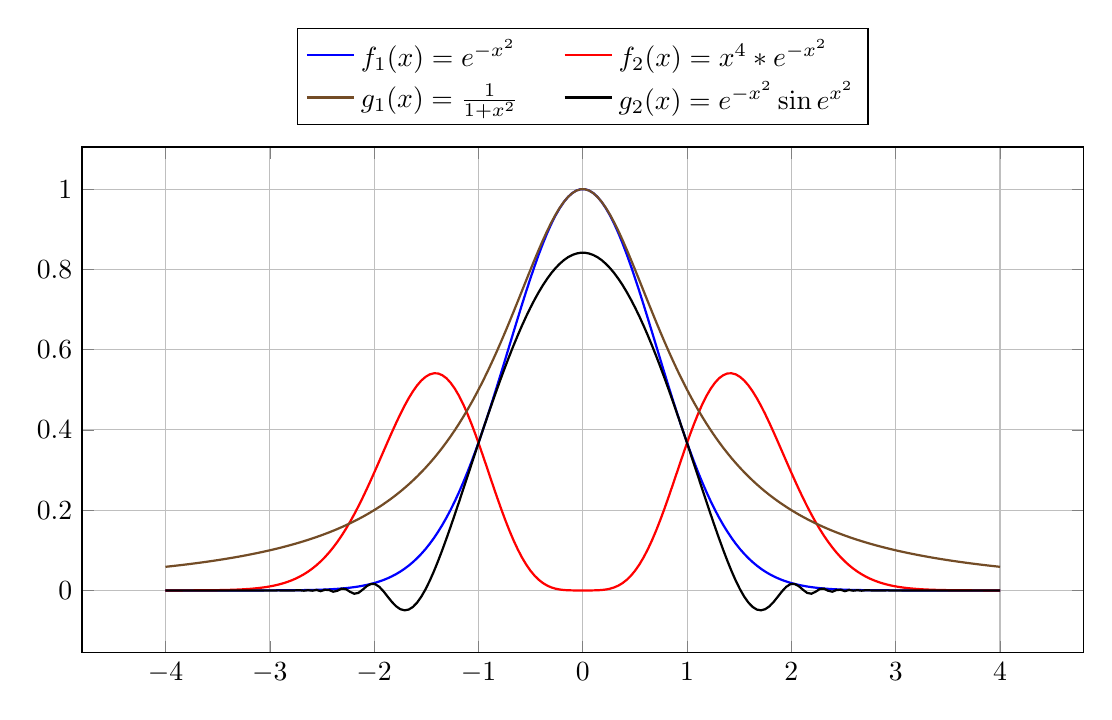
\begin{tikzpicture}
\begin{axis}[domain = -4:4, width = 14.3cm, height = 8cm, grid, legend cell align = left, legend style = { at = {(0.5, 1)}, legend columns = 2, anchor = south, yshift = 8pt, /tikz/every even column/.append style={column sep=0.5cm}}]
\addplot +[mark = none, samples=200, thick] {e^(- x^2)};
\addplot +[mark = none, samples=200, thick] {x^4 * e^(- x^2)};
\addplot +[mark = none, samples=200, thick] {1 / (1 + x^2)};
\addplot +[mark = none, samples=200, thick] {e^(-x^2) * sin(deg(e^(0.5 * x^2)))};

\addlegendentry{$f_1(x) = e^{-x^2}$}
\addlegendentry{$f_2(x) = x^4 * e^{-x^2}$}
\addlegendentry{$g_1(x) = \frac{1}{1 + x^2}$}
\addlegendentry{$g_2(x) = e^{-x^2} \sin e^{x^2}$}

\end{axis}
\end{tikzpicture}
